\chapter{Centripetal Acceleration}
\label{phys:centripetal-acceleration}

\assumes{Similar triangles; velocity as a vector; acceleration as the rate of change of velocity; limits.}

\begin{center}
\begin{minipage}{0.5\textwidth}
\centering
\begin{tikzpicture}[scale=1.1]
    \def\R{2}
    \coordinate (O) at (0,0);
    \def\aOne{100}
    \def\aTwo{72}
    \coordinate (P1) at (\aOne:\R);
    \coordinate (P2) at (\aTwo:\R);

    \draw[thick] (O) circle (\R);
    \fill (O) circle (1.3pt);

    \draw[thick] (O) -- (P1) node[midway, above left] {$r$};
    \draw[thick] (O) -- (P2) node[midway, above right] {$r$};

    % tangent velocity vectors (perpendicular to radius, direction of travel)
    \draw[thick,->] (P1) -- ($(P1)+(\aOne+90:1.3)$) node[above] {$v_1$};
    \draw[thick,->] (P2) -- ($(P2)+(\aTwo+90:1.3)$) node[above right] {$v_2$};
\end{tikzpicture}
\end{minipage}%
\begin{minipage}{0.42\textwidth}
\centering
% --- Triangle A: angle relation theta ---
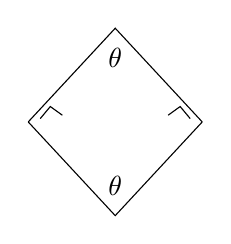
\begin{tikzpicture}[scale=0.85]
    \coordinate (Top) at (0,2);
    \coordinate (Left) at (-1.3,0.6);
    \coordinate (Right) at (1.3,0.6);
    \coordinate (Bottom) at (0,-0.8);
    \draw (Left) -- (Top) -- (Right);
    \draw (Left) -- (Bottom) -- (Right);
    \node at (0,1.55) {$\theta$};
    \node at (0,-0.35) {$\theta$};
    \draw (Left)++(0.18,0.05) -- ++(0.15,0.18) -- ++(0.18,-0.13);
    \draw (Right)++(-0.18,0.05) -- ++(-0.15,0.18) -- ++(-0.18,-0.13);
\end{tikzpicture}

\vspace{6pt}
% --- Triangle B: Delta v triangle ---
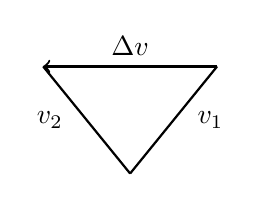
\begin{tikzpicture}[scale=0.85]
    \coordinate (Apex) at (0,0);
    \coordinate (TopLeft) at (-1.3,1.6);
    \coordinate (TopRight) at (1.3,1.6);
    \draw[thick] (Apex) -- (TopLeft);
    \draw[thick] (Apex) -- (TopRight);
    \draw[thick,->] (TopRight) -- (TopLeft);
    \node at (0,1.9) {$\Delta v$};
    \node at (-1.2,0.8) {$v_2$};
    \node at (1.2,0.8) {$v_1$};
\end{tikzpicture}

\vspace{6pt}
% --- Triangle C: Delta s triangle (same orientation as Delta v triangle above) ---
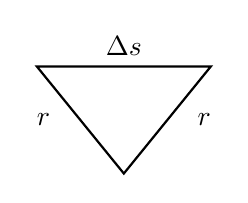
\begin{tikzpicture}[scale=0.85]
    \coordinate (Apex) at (0,0);
    \coordinate (TopLeft) at (-1.3,1.6);
    \coordinate (TopRight) at (1.3,1.6);
    \draw[thick] (Apex) -- (TopLeft) -- (TopRight) -- cycle;
    \node at (-1.2,0.8) {$r$};
    \node at (1.2,0.8) {$r$};
    \node at (0,1.9) {$\Delta s$};
\end{tikzpicture}
\end{minipage}
\end{center}

\noindent
Given the above, we can say:
\begin{equation}
\frac{\Delta v}{v_1} = \frac{\Delta s}{r}
\qquad
\therefore\; \Delta v = \frac{\Delta s \, v_1}{r}
\label{phys:eq:delta-v}
\end{equation}

\noindent
\textbf{Average acceleration:}
\[
a_{avg} = \frac{\Delta v}{\Delta t}
\]

\noindent
Substitute \eqref{phys:eq:delta-v} into the above:
\[
a_{avg} = \frac{\Delta s \, v_1}{\Delta t \, r}
\]

\[
a_{inst} = \lim_{\Delta t \to 0} \frac{\Delta s \, v_1}{\Delta t \, r}
\]

\noindent
We know that $\displaystyle\lim_{\Delta t \to 0} \frac{\Delta s}{\Delta t} = v = v_1$, therefore:
\[
a_{inst} = \frac{v_1 \cdot v_1}{r} = \frac{v_1^2}{r} = \frac{v^2}{r}
\]

\begin{center}
\boxed{\,a = \dfrac{v^2}{r}\,}
\end{center}

\bigskip
\noindent\textbf{Remark.} The derivation above only gives the \emph{magnitude} of the acceleration, but the direction is worth pointing out too: as $\Delta t \to 0$, the vector $\Delta \vec{v}$ rotates to point directly toward the centre $O$ of the circle -- which is exactly why this is called \emph{centripetal} acceleration, from the Latin \textit{centrum petere}, "to seek the centre." This resolves a common source of confusion: in uniform circular motion the \emph{speed} $v$ never changes, yet the object is still accelerating, because acceleration measures the rate of change of the \emph{velocity vector} -- and here it's the \emph{direction} of that vector that is constantly changing, not its length. Historically, this result predates Newton's \textit{Principia} (1687): Christiaan Huygens worked out the same formula around 1659, making it one of the earliest quantitative results in dynamics.
